\documentclass[a4paper,10pt,oneside]{article}

%\usepackage{ucs}
\usepackage[utf8]{inputenc}
%\usepackage{babel}
%\usepackage{fontenc}
\usepackage[pdftex]{graphicx}

\usepackage[dvips,pdftex]{hyperref}

\author{Cameron Robertson}
\date{11/09/17}

\begin{document}

\section{Introduction}
\label{sec:intro}

 In this section, the temperature
data from Uppsala will be analysed with the aid of histograms, which show the mean daily
temperatures from 1722 until 2013. Each histogram will show data for a specific day of the year,
so it may be enlightening to look at all 366 potential histograms, though this would
not be practical. Instead, a few specific dates will be chosen to analyse the histogram
distribution. It will then be determined how useful these results will be in determining the beginning
of Spring.

\section{Extracting the data}
\label{sec:data}

The Uppsala temperature data was given as a space seperated list, with the first three
columns representing the year, month and day respectively. The fourth column included the mean
temperature of that day unadjusted for urban effect, whereas the fifth column held
the same, but adjusted for urban effect. The temperatures to be plotted were those 
in the fifth column. The sixth held an id number to represent the weather station
that the temperature was recorded from. For the purposes of this project, only Uppsala
data was needed, which had an id of 1.

The function to extract the required information took two arguments: a day and a month. Firstly, each column was streamed into a vector. This was
easier and safer than using an array, since vectors dynamically change size. A for loop was then run which streamed the appropriate vector elements for the
chosen month and day into another file. This also only streamed the data with an id of 1. The data in the file was then streamed back into another
vector, which was then used to plot the histogram

\section{Results and Discussion}
\label{sec:res}

\begin{figure} 
  \begin{center}
    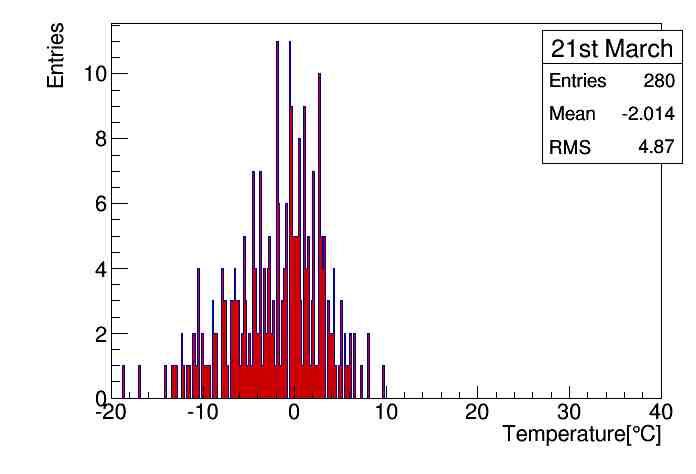
\includegraphics[width=10cm]{/home/courseuser/Project/Project/Code/Equinox_temps.jpg}
    \caption{Histogram showing temperatures from 1722-2013 at 21.3}
    \label{fig:vern}
  \end{center}
\end{figure}

Clearly \ref{fig:vern} shows that very generally, the temperature in Uppsala at the
vernal equinox tends to be below 0 degrees, which is colder than previously expected, especially given the previous
results from this report. However, the rather high standard deviation
shown in \ref{fig:vern} displays just how much variation in temperature there is over 300 years.
The range is also expectedly quite large, owing to the large quantity of data. Also, there have been several cases of extremely
cold temperatures, which could have altered the mean.

\begin{figure}
 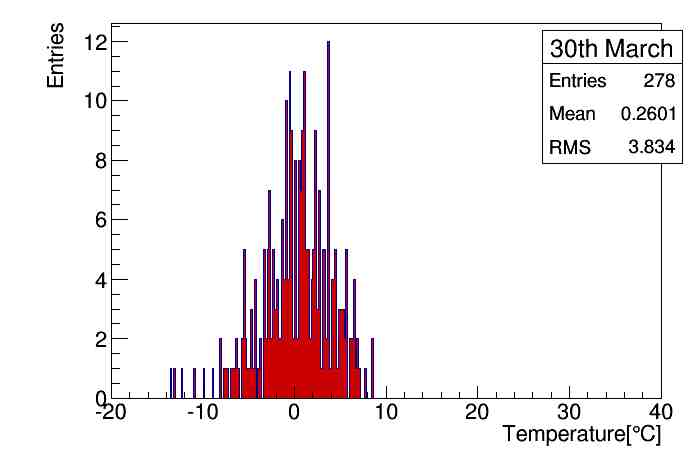
\includegraphics[width=10cm]{/home/courseuser/Project/Project/Code/week.jpg}
 \caption{Histogram showing temperatures from 1722-2013 at 30.3}
 \label{fig:week}
\end{figure}

Comparing \ref{fig:week} to \ref{fig:vern}, the mean temperature has clearly increased significantly even
after just one week, with the mean temperature now being above freezing. Notably, the standard deviation
has also decreased slightly, so the spread of results for this day is slightly lower than on the previous histogram, though is
still quite high.

\begin{figure}
 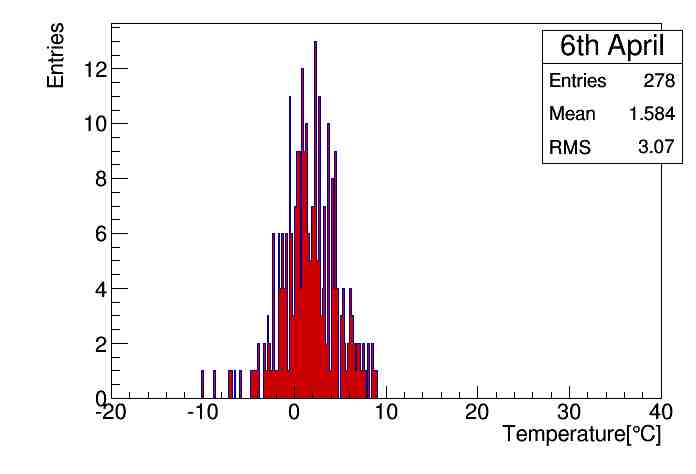
\includegraphics[width=10cm]{/home/courseuser/Project/Project/Code/2week.jpg}
 \caption{Histogram showing temperatures from 1722-2013 at 6.3}
 \label{fig:twoweek}
\end{figure}

The same trend continues one week on from this, as shown by \ref{fig:twoweek}. The mean temperature has again increased significantly
, though by a smaller value this time. Most notably, the spread of data has decreased, resulting in a visibly thinner histogram, resulting
in a lower standard deviation.

\section{Conclusion}
\label{sec:conc}

The results show that the large amount of data nevertheless still shows the expected trend of increasing temperature from week
to week, despite large standard deviation and recurring data from very cold years, which can be seen on
the left side of all the histograms. Theoretically, it would be possible to find the mean warmest and coldest day between 1722-2013,
but this would require repeatedly running the aforementioned function until the minimum and maximum values were found
It would also be difficult to determine the beginning of Spring(Using the temperature definition) using this program,
as a similar brute force method would be required, and it would be difficult to plot the results.






 
\end{document}
